\documentclass[a4paper,10pt]{article}
\usepackage[top=2cm, left = 2cm , right=2cm , bottom=2cm]{geometry}
\usepackage{amsmath}
\usepackage{amsfonts}
\usepackage[utf8]{inputenc}
\usepackage{amssymb}
\usepackage{graphicx}
\usepackage{float}
\usepackage{subcaption}
\usepackage[brazil]{babel}
%\pagestyle{plain}
\usepackage{listings}
\usepackage{color}
\usepackage{hyperref}
\usepackage{graphicx}

\definecolor{dkgreen}{rgb}{0,0.6,0}
\definecolor{gray}{rgb}{0.5,0.5,0.5}
\definecolor{mauve}{rgb}{0.58,0,0.82}

\lstset{frame=tb,
  language=bash,
  aboveskip=3mm,
  belowskip=3mm,
  showstringspaces=false,
  columns=flexible,
  basicstyle={\small\ttfamily},
  numbers=none,
  numberstyle=\tiny\color{gray},
  keywordstyle=\color{blue},
  commentstyle=\color{dkgreen},
  stringstyle=\color{mauve},
  breaklines=true,
  breakatwhitespace=true,
  tabsize=3,
  literate={á}{{\'a}}1
           {ç}{{\c{c}}}1
           {ü}{{\"u}}1
           {é}{{\'e}}1
}

\lstset{
}

\hypersetup{
    colorlinks=true,
    linkcolor=blue,
    filecolor=magenta,      
    urlcolor=cyan,
}
 
\urlstyle{same}

\begin{document}
%\twocolumn


\title{MC833 A - Programação de redes de computadores\\
Relatório - Projeto Final}

\author {   093125 - Tiago Martinho de Barros - \textit{tiago.ec09@gmail.com}\\
            093175 - Victor Fernando Pompêo Barbosa - \textit{victorfpb@gmail.com}}

%\date{}

\maketitle

\centerline{Prof. Paulo Lício de Geus}
\centerline{IC -- UNICAMP}

\vspace{2cm}
\tableofcontents
    
%%%%%%%%%%%%%%%%%%%%%%%%%%%%%%%%%%%%%%%%%%%%%%%%%%%%%%%%%%%%%%%%%%%%%%%%%%%%%
\newpage
\section{Introdução}
\hspace{14pt}

    Nesta tarefa modificaremos a aplicação Simplex-Talk desenvolvida anteriormente para incluir o suporte a múltiplos clientes simultaneamente.

%%%%%%%%%%%%%%%%%%%%%%%%%%%%%%%%%%%%%%%%%%%%%%%%%%%%%%%%%%%%%%%%%%%%%%%%%%%%%
\section{Questão 1}
A função {\tt getsockname} está definida em $\langle sys/socket.h \rangle$ e sua assinatura é:
    \begin{lstlisting}
    int getsockname(int sockfd, struct sockaddr *address, socklen_t *restrict address_len);
    \end{lstlisting}

Ela retorna o endereço atual a que o socket {\tt sockfd} está ligado, no buffer apontado por {\tt address}. O argumento {\tt address\_len} informa o espaço (em bytes) apontado por {\tt address}; quando a função retorna, {\tt address\_len} é sobrescrito com o tamanho real do endereço do socket.

Para que o programa {\tt client.c} passasse a obter os valores de IP e porta do socket local e os imprimisse na saída padrão, o seguinte trecho de código foi adicionado ao programa:

\begin{lstlisting}
    struct sockaddr_in local;
    unsigned int locallen;

    locallen = sizeof(local);
    if (getsockname(s, (struct sockaddr *)&local, &locallen) < 0) {
        perror("simplex-talk: getsockname");
        close(s);
        exit(1);
    }

    fprintf(stdout, "-------------------\n");
    fprintf(stdout, "IP local: %s\n", inet_ntoa(local.sin_addr));
    fprintf(stdout, "Porta local: %d\n", ntohs(local.sin_port));
    fprintf(stdout, "-------------------\n\n");

\end{lstlisting}

\section{Questão 2}
A função {\tt getpeername} está definida em $\langle sys/socket.h \rangle$ e sua assinatura é:
    \begin{lstlisting}
    int getpeername(int sockfd, struct sockaddr *address, socklen_t *restrict address_len);
    \end{lstlisting}

Ela retorna o endereço do peer conectado ao socket {\tt sockfd}, no buffer apontado por {\tt address}. O argumento {\tt address\_len} informa o espaço (em bytes) apontado por {\tt address}; quando a função retorna, {\tt address\_len} é sobrescrito com o tamanho real do endereço do socket.

Para que o programa {\tt server.c} passasse a obter os valores de IP e porta do socket local e os imprimisse na saída padrão, o seguinte trecho de código foi adicionado ao programa:

\begin{lstlisting}
    struct sockaddr_in peer;
    unsigned int peerlen;

    peerlen = sizeof(peer);
    if (getpeername(new_s, (struct sockaddr *)&peer, &peerlen) < 0) {
        perror("simplex-talk: getpeername");
        exit(1);
    }

    fprintf(stdout, "--------------------\n");
    fprintf(stdout, "IP remoto: %s\n", inet_ntoa(peer.sin_addr));
    fprintf(stdout, "Porta remota: %d\n", ntohs(peer.sin_port));
    fprintf(stdout, "--------------------\n\n");

\end{lstlisting}

\section{Questão 3}
Para que o servidor pudesse atender mais de um cliente, o loop principal foi alterado. A nova versão está copiada a seguir.

\begin{lstlisting}
for( ; ; ) {
                len = sizeof(sin);
        if ((new_s = accept(s, (struct sockaddr *)&sin, &len)) < 0) {
            perror("simplex-talk: accept");
            exit(1);
        }

        //do this if child
        if((pid = fork()) == 0) {
            close(s);

            peerlen = sizeof(peer);
            if (getpeername(new_s, (struct sockaddr *)&peer, &peerlen) < 0) {
                perror("simplex-talk: getpeername");
                exit(1);
            }

            fprintf(stdout, "--------------------\n");
            fprintf(stdout, "IP remoto: %s\n", inet_ntoa(peer.sin_addr));
            fprintf(stdout, "Porta remota: %d\n", ntohs(peer.sin_port));
            fprintf(stdout, "My process ID : %d\n", getpid());
            fprintf(stdout, "My parent's ID: %d\n", getppid());

            fprintf(stdout, "--------------------\n\n");

            while ((len = recv(new_s, buf, sizeof(buf), 0))) {
                fputs(buf, stdout);
                if ((send(new_s, buf, strlen(buf)+1, 0)) < 0) {
                    perror("simplex-talk: send");
                    exit(1);
                }
            }

            //close child connection
            close(new_s);
            exit(0);
        }

        //close parent connection (the child owns this socket now)
        close(new_s);

    }
    
\end{lstlisting}

O primeiro trecho aceita uma nova conexão; em seguida, o processo pai utiliza {\tt fork} para criar processos filhos. A função {\tt fork} tem dois tipos de retorno diferentes, no caso de sucesso: para o pai, ela retorna o PID do filho; para o filho, ela retorna zero. Dessa maneira, o trecho {\tt if((pid = fork()) == 0)} certifica-se que aquele bloco de código apenas será executado pelo processo filho (já que o pai só será utilizado para distribuir as conexões).

O bloco de código seguinte lida com a conexão da mesma forma que o Simplex-talk não concorrente, com as modificações propostas pela Questão 1.

Por fim, o processo filho fecha a conexão estabelecida antes de invocar {\tt exit(0)}.

\section{Questão 4}
No início do bloco de código {\tt if} que é executado apenas no processo filho, o comando {\tt close(s)} fecha o descritor de arquivo do socket utilizado pelo processo pai, já que, quando {\tt fork} foi invocada, os descritores foram duplicados. Dessa maneira, o processo pai não perde acesso ao descritor. Antes de invocar {\tt exit(0)}, o filho também fecha o descritor do socket que estava utilizando.

De maneira similar, após passar o controle da conexão ao processo filho, o pai utiliza {\tt close(new\_s)} para fechar o descritor de arquivo do socket que passou a ser utilizado pelo filho.

\section{Questão 5}
O servidor foi inicializado, recebendo conexões de 3 clientes diferentes. A saída do terminal referente ao processo do servidor está exibida a seguir.

\begin{lstlisting}
niko@ubuntu:~/Desktop/mc833/t4$ ./server 
Server process ID : 8749
--------------------
IP remoto: 127.0.0.1
Porta remota: 45026
My process ID : 8751
My parent's ID: 8749
--------------------

--------------------
IP remoto: 127.0.0.1
Porta remota: 45027
My process ID : 8753
My parent's ID: 8749
--------------------

--------------------
IP remoto: 127.0.0.1
Porta remota: 45028
My process ID : 8755
My parent's ID: 8749
--------------------

Este é o cliente 1
Este é o cliente 2
Este é o cliente 3
Mensagem1
Mensagem do cliente 2
Mensagem um pouco maior vinda do cliente 3

\end{lstlisting}

A saída referente ao primeiro cliente pode ser verificada a seguir.

\begin{lstlisting}
niko@ubuntu:~/Desktop/mc833/t4$ ./client localhost
-------------------
IP local: 127.0.0.1
Porta local: 45026
-------------------

Este é o cliente 1
Este é o cliente 1

Mensagem1
Mensagem1

\end{lstlisting}

A saída referente ao segundo cliente foi copiada a seguir.

\begin{lstlisting}
niko@ubuntu:~/Desktop/mc833/t4$ ./client localhost
-------------------
IP local: 127.0.0.1
Porta local: 45027
-------------------

Este é o cliente 2
Este é o cliente 2

Mensagem do cliente 2
Mensagem do cliente 2

\end{lstlisting}

A saída referente ao terceiro cliente está exibida a seguir.

\begin{lstlisting}
niko@ubuntu:~/Desktop/mc833/t4$ ./client localhost
-------------------
IP local: 127.0.0.1
Porta local: 45028
-------------------

Este é o cliente 3
Este é o cliente 3

Mensagem um pouco maior vinda do cliente 3
Mensagem um pouco maior vinda do cliente 3

\end{lstlisting}

Com auxílio do comando {\tt tcpdump}, pode-se verificar a simultaneidade da comunicação. A saída do comando está listada a seguir.

\begin{lstlisting}
niko@ubuntu:~/Desktop/mc833/t4$ sudo tcpdump -i lo
tcpdump: verbose output suppressed, use -v or -vv for full protocol decode
listening on lo, link-type EN10MB (Ethernet), capture size 262144 bytes
05:49:26.823260 IP localhost.47273 > ubuntu.domain: 14274+ A? 9.client-channel.google.com. (45)
05:49:26.823400 IP localhost.47273 > ubuntu.domain: 569+ AAAA? 9.client-channel.google.com. (45)
05:49:26.826927 IP ubuntu.domain > localhost.47273: 14274 1/0/0 A 64.233.186.189 (61)
05:49:26.880994 IP ubuntu.domain > localhost.47273: 569 1/0/0 AAAA 2800:3f0:4003:c00::bd (73)
05:49:31.087009 IP localhost.45026 > localhost.31472: Flags [P.], seq 3964889944:3964889965, ack 1531317466, win 342, options [nop,nop,TS val 30456659 ecr 30454169], length 21
05:49:31.087033 IP localhost.31472 > localhost.45026: Flags [.], ack 21, win 342, options [nop,nop,TS val 30456659 ecr 30456659], length 0
05:49:31.087067 IP localhost.31472 > localhost.45026: Flags [P.], seq 1:22, ack 21, win 342, options [nop,nop,TS val 30456659 ecr 30456659], length 21
05:49:31.087075 IP localhost.45026 > localhost.31472: Flags [.], ack 22, win 342, options [nop,nop,TS val 30456659 ecr 30456659], length 0
05:49:35.728454 IP localhost.45027 > localhost.31472: Flags [P.], seq 639206581:639206602, ack 1142775101, win 342, options [nop,nop,TS val 30457819 ecr 30454468], length 21
05:49:35.728475 IP localhost.31472 > localhost.45027: Flags [.], ack 21, win 342, options [nop,nop,TS val 30457819 ecr 30457819], length 0
05:49:35.728504 IP localhost.31472 > localhost.45027: Flags [P.], seq 1:22, ack 21, win 342, options [nop,nop,TS val 30457819 ecr 30457819], length 21
05:49:35.728511 IP localhost.45027 > localhost.31472: Flags [.], ack 22, win 342, options [nop,nop,TS val 30457819 ecr 30457819], length 0
05:49:39.705846 IP localhost.45028 > localhost.31472: Flags [P.], seq 746461835:746461856, ack 1805666008, win 342, options [nop,nop,TS val 30458814 ecr 30454754], length 21
05:49:39.705869 IP localhost.31472 > localhost.45028: Flags [.], ack 21, win 342, options [nop,nop,TS val 30458814 ecr 30458814], length 0
05:49:39.705903 IP localhost.31472 > localhost.45028: Flags [P.], seq 1:22, ack 21, win 342, options [nop,nop,TS val 30458814 ecr 30458814], length 21
05:49:39.705910 IP localhost.45028 > localhost.31472: Flags [.], ack 22, win 342, options [nop,nop,TS val 30458814 ecr 30458814], length 0
05:49:42.756102 IP localhost.45026 > localhost.31472: Flags [P.], seq 21:32, ack 22, win 342, options [nop,nop,TS val 30459576 ecr 30456659], length 11
05:49:42.756138 IP localhost.31472 > localhost.45026: Flags [P.], seq 22:33, ack 32, win 342, options [nop,nop,TS val 30459576 ecr 30459576], length 11
05:49:42.756148 IP localhost.45026 > localhost.31472: Flags [.], ack 33, win 342, options [nop,nop,TS val 30459576 ecr 30459576], length 0
05:49:48.823189 IP localhost.45027 > localhost.31472: Flags [P.], seq 21:44, ack 22, win 342, options [nop,nop,TS val 30461093 ecr 30457819], length 23
05:49:48.823224 IP localhost.31472 > localhost.45027: Flags [P.], seq 22:45, ack 44, win 342, options [nop,nop,TS val 30461093 ecr 30461093], length 23
05:49:48.823233 IP localhost.45027 > localhost.31472: Flags [.], ack 45, win 342, options [nop,nop,TS val 30461093 ecr 30461093], length 0
05:49:53.748444 IP localhost.58669 > ubuntu.domain: 34560+ A? ads.papeeria.com. (34)
05:49:53.748648 IP localhost.58669 > ubuntu.domain: 20558+ AAAA? ads.papeeria.com. (34)
05:49:53.749248 IP localhost.36247 > ubuntu.domain: 30102+ A? papeeria.com. (30)
05:49:53.749346 IP localhost.36247 > ubuntu.domain: 52510+ AAAA? papeeria.com. (30)
05:49:53.750965 IP localhost.57545 > ubuntu.domain: 1295+ A? papeeria-alert.blogspot.com. (45)
05:49:53.751033 IP localhost.57545 > ubuntu.domain: 56816+ AAAA? papeeria-alert.blogspot.com. (45)
05:49:53.751322 IP localhost.58544 > ubuntu.domain: 48779+ A? papeeria-alert.blogspot.com. (45)
05:49:53.754663 IP ubuntu.domain > localhost.57545: 1295 2/0/0 CNAME blogspot.l.googleusercontent.com., A 216.58.202.1 (104)
05:49:53.889355 IP ubuntu.domain > localhost.58669: 20558 0/1/0 (124)
05:49:53.892601 IP ubuntu.domain > localhost.58669: 34560 1/0/0 A 104.155.12.58 (50)
05:49:53.893628 IP ubuntu.domain > localhost.36247: 30102 1/0/0 A 104.155.84.196 (46)
05:49:54.810174 IP localhost.45028 > localhost.31472: Flags [P.], seq 21:65, ack 22, win 342, options [nop,nop,TS val 30462590 ecr 30458814], length 44
05:49:54.810221 IP localhost.31472 > localhost.45028: Flags [P.], seq 22:66, ack 65, win 342, options [nop,nop,TS val 30462590 ecr 30462590], length 44
05:49:54.810252 IP localhost.45028 > localhost.31472: Flags [.], ack 66, win 342, options [nop,nop,TS val 30462590 ecr 30462590], length 0
05:49:55.749579 IP ubuntu.domain > localhost.36247: 52510 0/1/0 (120)
05:49:55.751468 IP ubuntu.domain > localhost.57545: 56816 2/0/0 CNAME blogspot.l.googleusercontent.com., AAAA 2800:3f0:4001:803::2001 (116)
05:49:55.807040 IP ubuntu.domain > localhost.58544: 48779 2/0/0 CNAME blogspot.l.googleusercontent.com., A 216.58.202.97 (104)
^C
39 packets captured
78 packets received by filter
0 packets dropped by kernel

\end{lstlisting}

Suprimindo as linhas referentes a conexões de outros processos, podemos analisar melhor a comunicação entre servidor/cliente de nosso Simplex-Talk.

\begin{lstlisting}
niko@ubuntu:~/Desktop/mc833/t4$ sudo tcpdump -i lo
tcpdump: verbose output suppressed, use -v or -vv for full protocol decode
listening on lo, link-type EN10MB (Ethernet), capture size 262144 bytes
05:49:31.087009 IP localhost.45026 > localhost.31472: Flags [P.], seq 3964889944:3964889965, ack 1531317466, win 342, options [nop,nop,TS val 30456659 ecr 30454169], length 21
05:49:31.087033 IP localhost.31472 > localhost.45026: Flags [.], ack 21, win 342, options [nop,nop,TS val 30456659 ecr 30456659], length 0
05:49:31.087067 IP localhost.31472 > localhost.45026: Flags [P.], seq 1:22, ack 21, win 342, options [nop,nop,TS val 30456659 ecr 30456659], length 21
05:49:31.087075 IP localhost.45026 > localhost.31472: Flags [.], ack 22, win 342, options [nop,nop,TS val 30456659 ecr 30456659], length 0
05:49:35.728454 IP localhost.45027 > localhost.31472: Flags [P.], seq 639206581:639206602, ack 1142775101, win 342, options [nop,nop,TS val 30457819 ecr 30454468], length 21
05:49:35.728475 IP localhost.31472 > localhost.45027: Flags [.], ack 21, win 342, options [nop,nop,TS val 30457819 ecr 30457819], length 0
05:49:35.728504 IP localhost.31472 > localhost.45027: Flags [P.], seq 1:22, ack 21, win 342, options [nop,nop,TS val 30457819 ecr 30457819], length 21
05:49:35.728511 IP localhost.45027 > localhost.31472: Flags [.], ack 22, win 342, options [nop,nop,TS val 30457819 ecr 30457819], length 0
05:49:39.705846 IP localhost.45028 > localhost.31472: Flags [P.], seq 746461835:746461856, ack 1805666008, win 342, options [nop,nop,TS val 30458814 ecr 30454754], length 21
05:49:39.705869 IP localhost.31472 > localhost.45028: Flags [.], ack 21, win 342, options [nop,nop,TS val 30458814 ecr 30458814], length 0
05:49:39.705903 IP localhost.31472 > localhost.45028: Flags [P.], seq 1:22, ack 21, win 342, options [nop,nop,TS val 30458814 ecr 30458814], length 21
05:49:39.705910 IP localhost.45028 > localhost.31472: Flags [.], ack 22, win 342, options [nop,nop,TS val 30458814 ecr 30458814], length 0
05:49:42.756102 IP localhost.45026 > localhost.31472: Flags [P.], seq 21:32, ack 22, win 342, options [nop,nop,TS val 30459576 ecr 30456659], length 11
05:49:42.756138 IP localhost.31472 > localhost.45026: Flags [P.], seq 22:33, ack 32, win 342, options [nop,nop,TS val 30459576 ecr 30459576], length 11
05:49:42.756148 IP localhost.45026 > localhost.31472: Flags [.], ack 33, win 342, options [nop,nop,TS val 30459576 ecr 30459576], length 0
05:49:48.823189 IP localhost.45027 > localhost.31472: Flags [P.], seq 21:44, ack 22, win 342, options [nop,nop,TS val 30461093 ecr 30457819], length 23
05:49:48.823224 IP localhost.31472 > localhost.45027: Flags [P.], seq 22:45, ack 44, win 342, options [nop,nop,TS val 30461093 ecr 30461093], length 23
05:49:48.823233 IP localhost.45027 > localhost.31472: Flags [.], ack 45, win 342, options [nop,nop,TS val 30461093 ecr 30461093], length 0
05:49:54.810174 IP localhost.45028 > localhost.31472: Flags [P.], seq 21:65, ack 22, win 342, options [nop,nop,TS val 30462590 ecr 30458814], length 44
05:49:54.810221 IP localhost.31472 > localhost.45028: Flags [P.], seq 22:66, ack 65, win 342, options [nop,nop,TS val 30462590 ecr 30462590], length 44
05:49:54.810252 IP localhost.45028 > localhost.31472: Flags [.], ack 66, win 342, options [nop,nop,TS val 30462590 ecr 30462590], length 0
^C
39 packets captured
78 packets received by filter
0 packets dropped by kernel

\end{lstlisting}

Como pode-se verificar, a comunicação se dá exatamente entre as portas utilizadas pelo servidor e por cada um dos processos clientes, e possuem exatamente o mesmo tamanho das mensagens enviadas.

Para verificar que os processos criados para manipular cada conexão individual do servidor aos clientes são filhos do processo original, o código de {\tt server.c} foi modificado para contar com o auxílio das funções {\tt getpid()}, que retorna o PID do processo atual; e {\tt getppid()}, que retorna o PID do processo pai. Antes de entrar no laço principal, o processo do servidor imprime na tela seu PID:

\begin{lstlisting}
    fprintf(stdout, "Server process ID : %d\n", getpid());

\end{lstlisting}

E, dentro do laço principal, ao mesmo tempo em que o processo filho verifica o IP e a porta remotos, ele imprime seu PID e o PID de seu processo pai:

\begin{lstlisting}
            fprintf(stdout, "--------------------\n");
            fprintf(stdout, "IP remoto: %s\n", inet_ntoa(peer.sin_addr));
            fprintf(stdout, "Porta remota: %d\n", ntohs(peer.sin_port));
            fprintf(stdout, "My process ID : %d\n", getpid());
            fprintf(stdout, "My parent's ID: %d\n", getppid());
            fprintf(stdout, "--------------------\n\n");

\end{lstlisting}

Observando a saída do servidor, pode-se verificar que seu PID é retornado corretamente todas as vezes que os processos filhos invocam {\tt getppid()}.

\begin{lstlisting}
niko@ubuntu:~/Desktop/mc833/t4$ ./server 
Server process ID : 8749
--------------------
IP remoto: 127.0.0.1
Porta remota: 45026
My process ID : 8751
My parent's ID: 8749
--------------------

--------------------
IP remoto: 127.0.0.1
Porta remota: 45027
My process ID : 8753
My parent's ID: 8749
--------------------

--------------------
IP remoto: 127.0.0.1
Porta remota: 45028
My process ID : 8755
My parent's ID: 8749
--------------------

Este é o cliente 1
Este é o cliente 2
Este é o cliente 3
Mensagem1
Mensagem do cliente 2
Mensagem um pouco maior vinda do cliente 3

\end{lstlisting}

\section{Questão 6}

Para resolver esta questão, podemos utilizar a ferramenta {\tt netstat}, que exibe as conexões ativas.

Vamos usar um novo exemplo, com o servidor:

\begin{lstlisting}
Server process ID : 13387
--------------------
IP remoto: 127.0.0.1
Porta remota: 41952
My process ID : 13392
My parent's ID: 13387
--------------------
\end{lstlisting}

e o cliente:

\begin{lstlisting}
Server process ID : 13387
-------------------
IP local: 127.0.0.1
Porta local: 41952
-------------------
\end{lstlisting}

e a saída do comando {\tt netstat -tu} (mostrando as linhas relevantes):

\begin{lstlisting}
tcp        0      0 localhost.localdo:41952 localhost.localdo:31472 ESTABLISHED
tcp        0      0 localhost.localdo:31472 localhost.localdo:41952 ESTABLISHED
\end{lstlisting}

Quando se fecha o cliente, a saída de {\tt netstat -tu} fica:

\begin{lstlisting}
tcp        0      0 localhost.localdo:41952 localhost.localdo:31472 TIME_WAIT
\end{lstlisting}

mostrando que o cliente fica no estado \textbf{TIME\_WAIT} após o encerramento da conexão.
Porém, se o servidor for fechado antes do cliente, é o servidor que fica no estado \textbf{TIME\_WAIT}. Ou seja, o primeiro a ser fechado entra no estado \textbf{TIME\_WAIT}.
O que condiz com a figura~\ref{fig:tcpstates}\footnote{Fonte: http://www4.cs.fau.de/Projects/JX/Projects/TCP/tcpstate.gif}, que considera que o cliente fecha a conexão ativamente.

\begin{figure}[htb]
    \begin{center}
	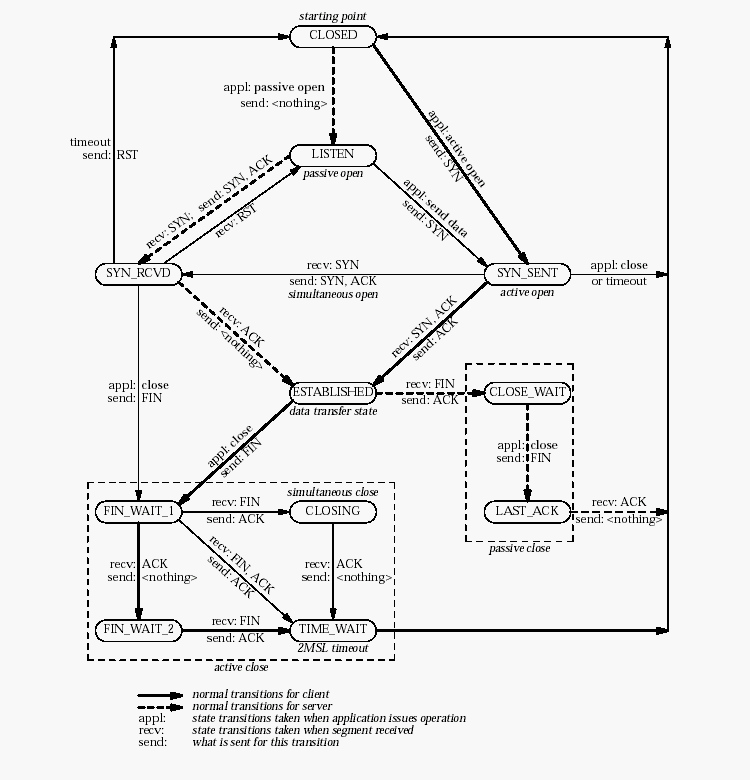
\includegraphics[width=\textwidth]{tcpstate.png}
	\caption{Estados do TCP}
	\label{fig:tcpstates}
	\end{center}
\end{figure}

Essa situação condiz com a implementação, pois o primeiro que fechar a conexão, chamando a função {\tt close}, não enviará mais nada, porém pode haver pacotes do nó remoto (\textit{peer}) que pertencem a essa conexão. Se \textbf{TIME\_WAIT} não existir, uma nova conexão pode ser feita com os mesmos endereços IP e mesmas portas e esta nova conexão poderá receber pacotes da conexão antiga, caso haja, o que não é uma coisa desejável, normalmente. O período em que se fica no estado \textbf{TIME\_WAIT} é 2 MSL, sendo MSL o \textit{Maximum Segment Lifetime}, tempo máximo em que um segmento fica válido. Outro motivo para o estado \textbf{TIME\_WAIT} é para implementar o fechamento confiável de conexão full-duplex do TCP, pois o FIN pode ser reenviado caso o ACK do outro nó se perca.

\end{document}

